% Created 2024-06-20 Thu 20:06
% Intended LaTeX compiler: pdflatex
\documentclass[11pt]{article}
\usepackage[utf8]{inputenc}
\usepackage[T1]{fontenc}
\usepackage{graphicx}
\usepackage{longtable}
\usepackage{wrapfig}
\usepackage{rotating}
\usepackage[normalem]{ulem}
\usepackage{amsmath}
\usepackage{amssymb}
\usepackage{capt-of}
\usepackage{hyperref}
\synctex=1
\usepackage[margin=1in]{geometry}
\usepackage{graphicx}
\usepackage{amsmath,bm}
\usepackage{algpseudocode}
\usepackage[ruled,vlined]{algorithm2e}
\usepackage[version=4]{mhchem}
\usepackage{siunitx}
\usepackage{longtable,tabularx}
\usepackage{booktabs}
\usepackage{tabularx,longtable,multirow,subfigure,caption}
\setlength\LTleft{0pt}
\usepackage{mathrsfs}
\usepackage{amsfonts}
\usepackage{enumitem}
\usepackage{mathalpha}
\renewcommand{\figurename}{\bf \small Figure}
\renewcommand{\tablename}{\bf \small Table}
\newcommand{\de}{\delta}
\newcommand{\ve}{\text{v}}
\newcommand{\lo}{\mathcal{L}}
\newcommand{\vt}{\overline{\delta\bm{\theta}}}
\newcommand{\vu}{\overline{\delta\bm{u}}}
\newcommand{\e}{\bm{\mathfrak{e}}}
\newcommand{\E}{\bm{\mathbb{E}}}
\newcommand{\T}{\bm{\mathcal{T}}}
\newcommand{\fra}{(\mathtt{1})}
\newcommand{\frb}{(\mathtt{2})}
\newcommand{\fri}{(\mathfrak{i})}
\newcommand{\bs}[1]{\boldsymbol{#1}}
\newcommand{\rhoinf}{\rho}
\newcommand{\Vinf}{U}
\newcommand{\Cl}[1]{c_{l_{#1}}}
\newcommand{\barCl}[1]{\bar{c}_{l_{#1}}}
\newcommand{\Cm}[1]{c_{m_{#1}}}
\newcommand{\barCm}[1]{\bar{c}_{m_{#1}}}
\newcommand{\AIC}{\bs{\mathcal{A}}}
\author{Alvaro Cea and Rafael Palacios}
\date{\today}
\title{Geometrically Nonlinear Analysis of Flexible Aircraft on Modern Hardware Architectures}
\hypersetup{
 pdfauthor={Alvaro Cea and Rafael Palacios},
 pdftitle={Geometrically Nonlinear Analysis of Flexible Aircraft on Modern Hardware Architectures},
 pdfkeywords={},
 pdfsubject={},
 pdfcreator={Emacs 29.1 (Org mode 9.6.6)}, 
 pdflang={English}}
\begin{document}

\maketitle

\begin{abstract}
This paper presents a new simulation environment for time-domain nonlinear aeroelastic analysis built for performance and that is suitable for modern hardware architectures such as GPUs.
The numerical library JAX and a novel description of the aircraft dynamics are brought together into a highly vectorised codebase that achieves two orders of magnitude accelerations compare to conventional implementations. This brings full-vehicle simulations to run close to if not in real-time, thus opening new possibilities for aircraft aeroelastic analysis which have traditionally been constrained to either linear, frequency domain solutions, or to their nonlinear counterparts but narrower in scope. Moreover, the approach seamlessly integrates with conventional aeroelastic load packages which facilitates the analysis of complex aircraft configurations.
A large test suite of problems has been built for the validation and maintainability of the code, which includes static and dynamic, structural and aeroelastic examples. A summary is presented herein along side a computational benchmark on CPUs and GPUs.
The nonlinear trim and gust response of an industrial configuration are studied and illustrate the capabilities of the proposed approach. Verification against MSC Nastran is shown first for small deformations, to then highlight the main differences between linear and nonlinear analysis for very high loading scenarios that induce large displacements. We show our nonlinear, time-domain solver outperforms linear Nastran in computational speed. 
\end{abstract}

\section{Results}
\label{sec:org2660cd0}
\subsection{Canonical case: unsupported dynamics of very flexible structure}
\label{sec:orge08446a}
This example exemplifies the ability of our solvers to turn a generic linear free-free finite-element model into a fully nonlinear solution that accounts for the rigid-body dynamics coupled with large elastic deformations. It has already been presented in \cite{PALACIOS2019}, though the novelties introduced herein are the new optimised implementation that can run on accelerators and the approach to recover the full 3D state from the reduced model.
The beam version of this structure was first studied by Simo and Vu-Quoc \cite{SIMO1988} and has served to verify several implementations of nonlinear beam dynamics with rigid body motions \cite{HESSE2014}.
A straight structure of constant square cross section (side = 3, wall thickness = 3/10) is built consisting of 784 shell elements linked to 50 spanwise nodes via interpolation elements as depicted in Fig. \ref{fig:org248a372} together with the material properties and two types of loading: firstly, a dead-force in the x-direction and dead-moment in the z-direction that yield a planar motion in the x-y plane; and secondly, the addition of a moment in the y-direction which produces a three dimensional motion.

\begin{figure}[htbp]
\centering
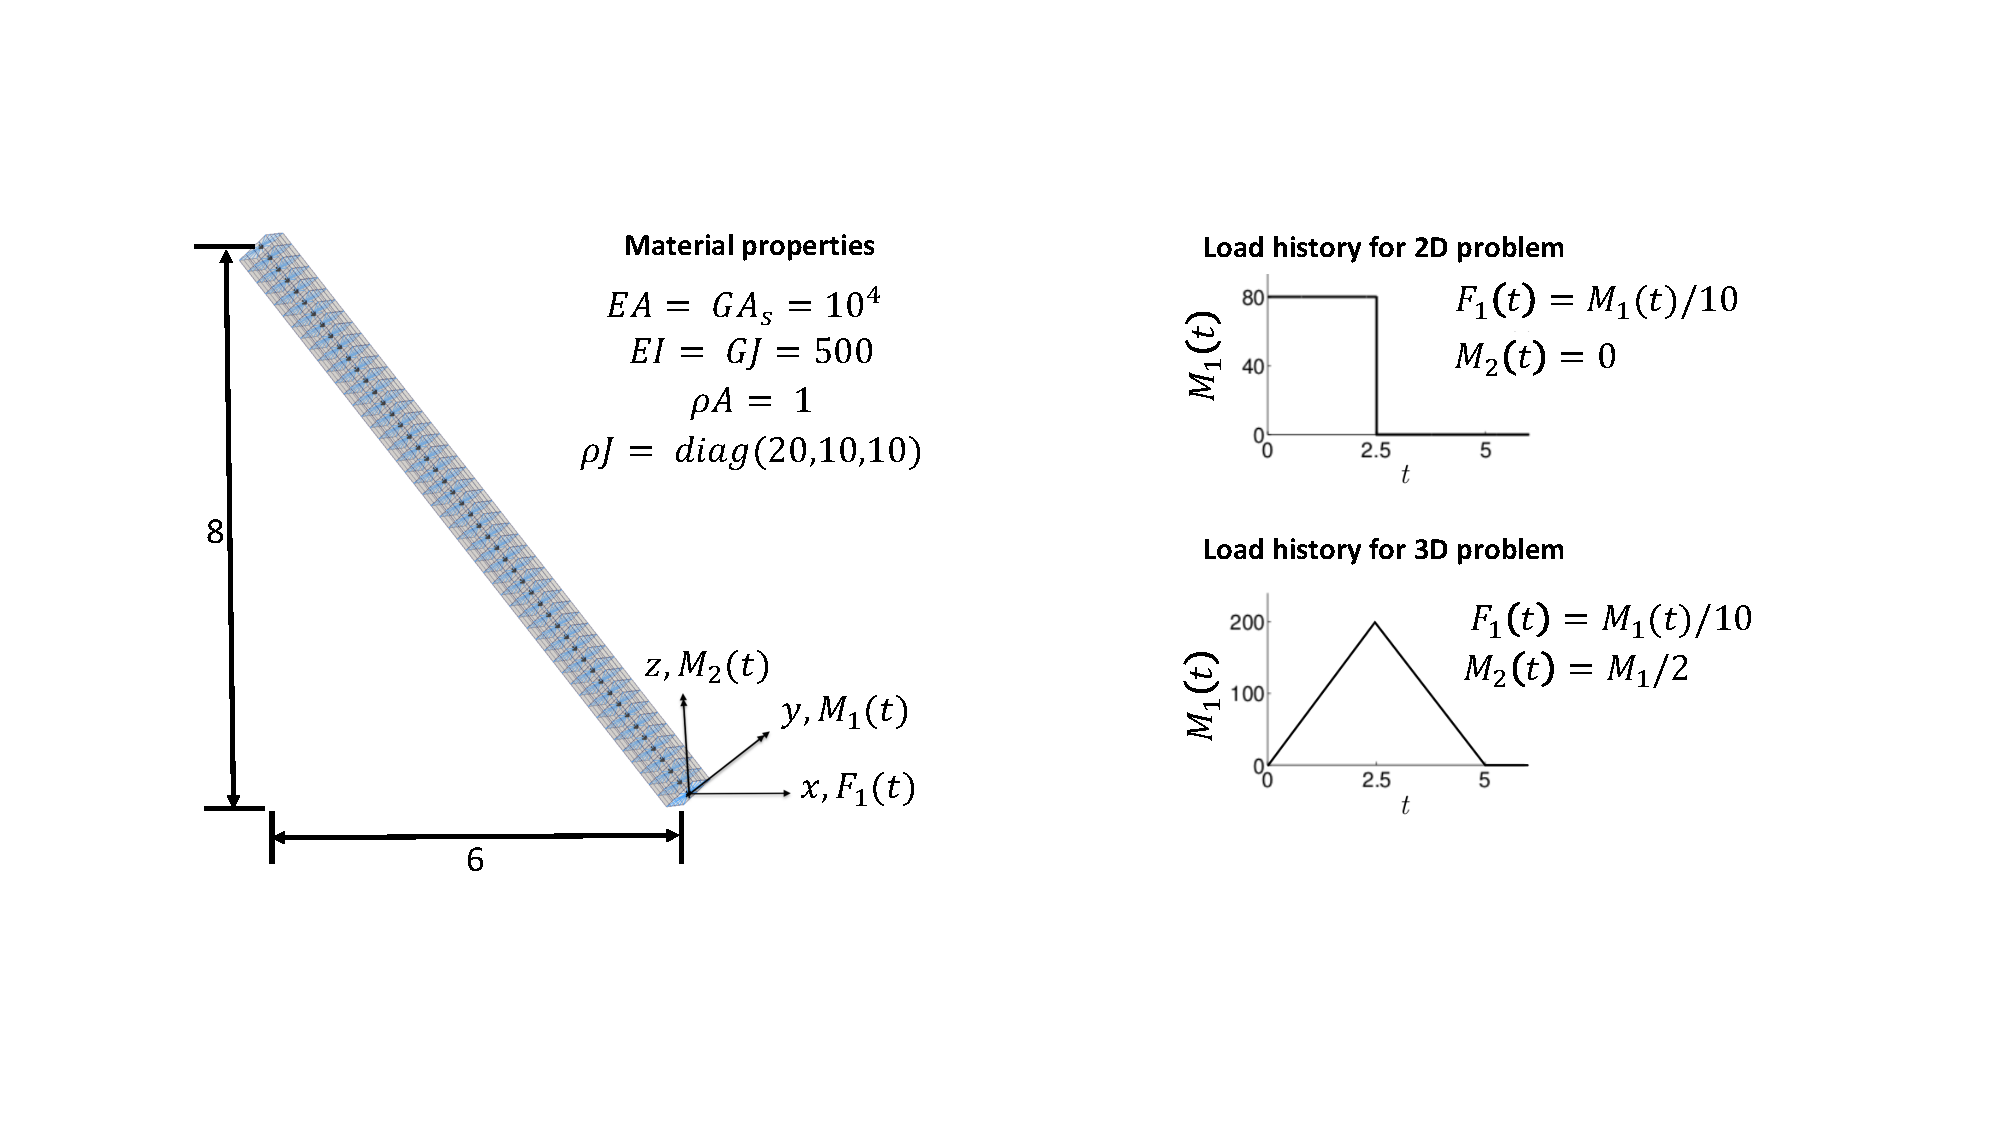
\includegraphics[width=0.7\textwidth]{figs_ext/ffbw10.pdf}
\caption{\label{fig:org248a372}FFS geometry, material properties and load cases}
\end{figure}

The free-flying evolution of the 3D model is shown in Fig. \ref{fig:org9faf760} for the planar motion and Fig. \ref{fig:org6578e1b} for the loads giving rise to the full 3D deformations. It worth remarking the latter motion also exhibits large torsional deformations which are combined with the also large bending displacements and rigid-body modes.

\begin{figure}[htbp]
\centering
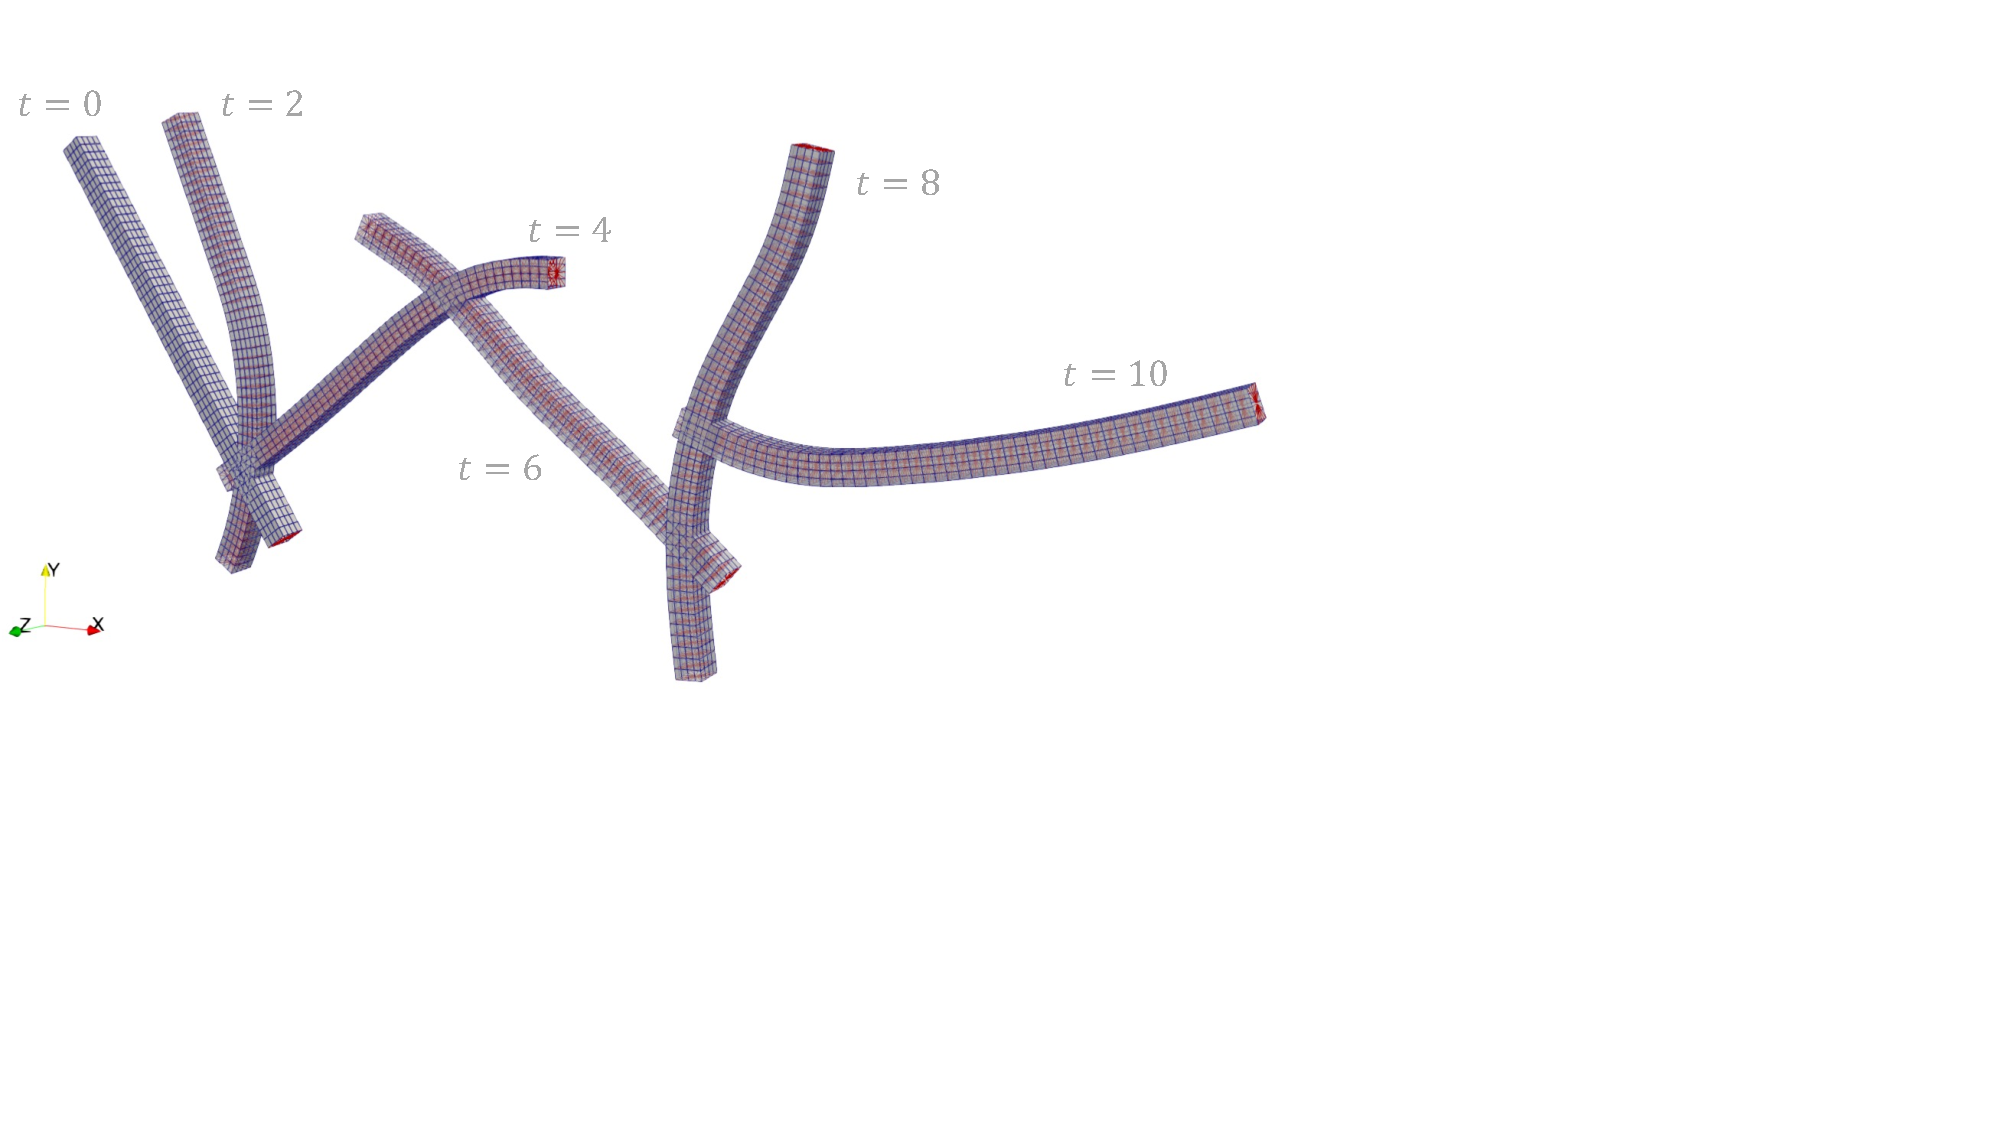
\includegraphics[width=0.8\textwidth]{figs_ext/FFB_2D3.pdf}
\caption{\label{fig:org9faf760}Free-flying structure in the 2D plane}
\end{figure}


\begin{figure}[htbp]
\centering
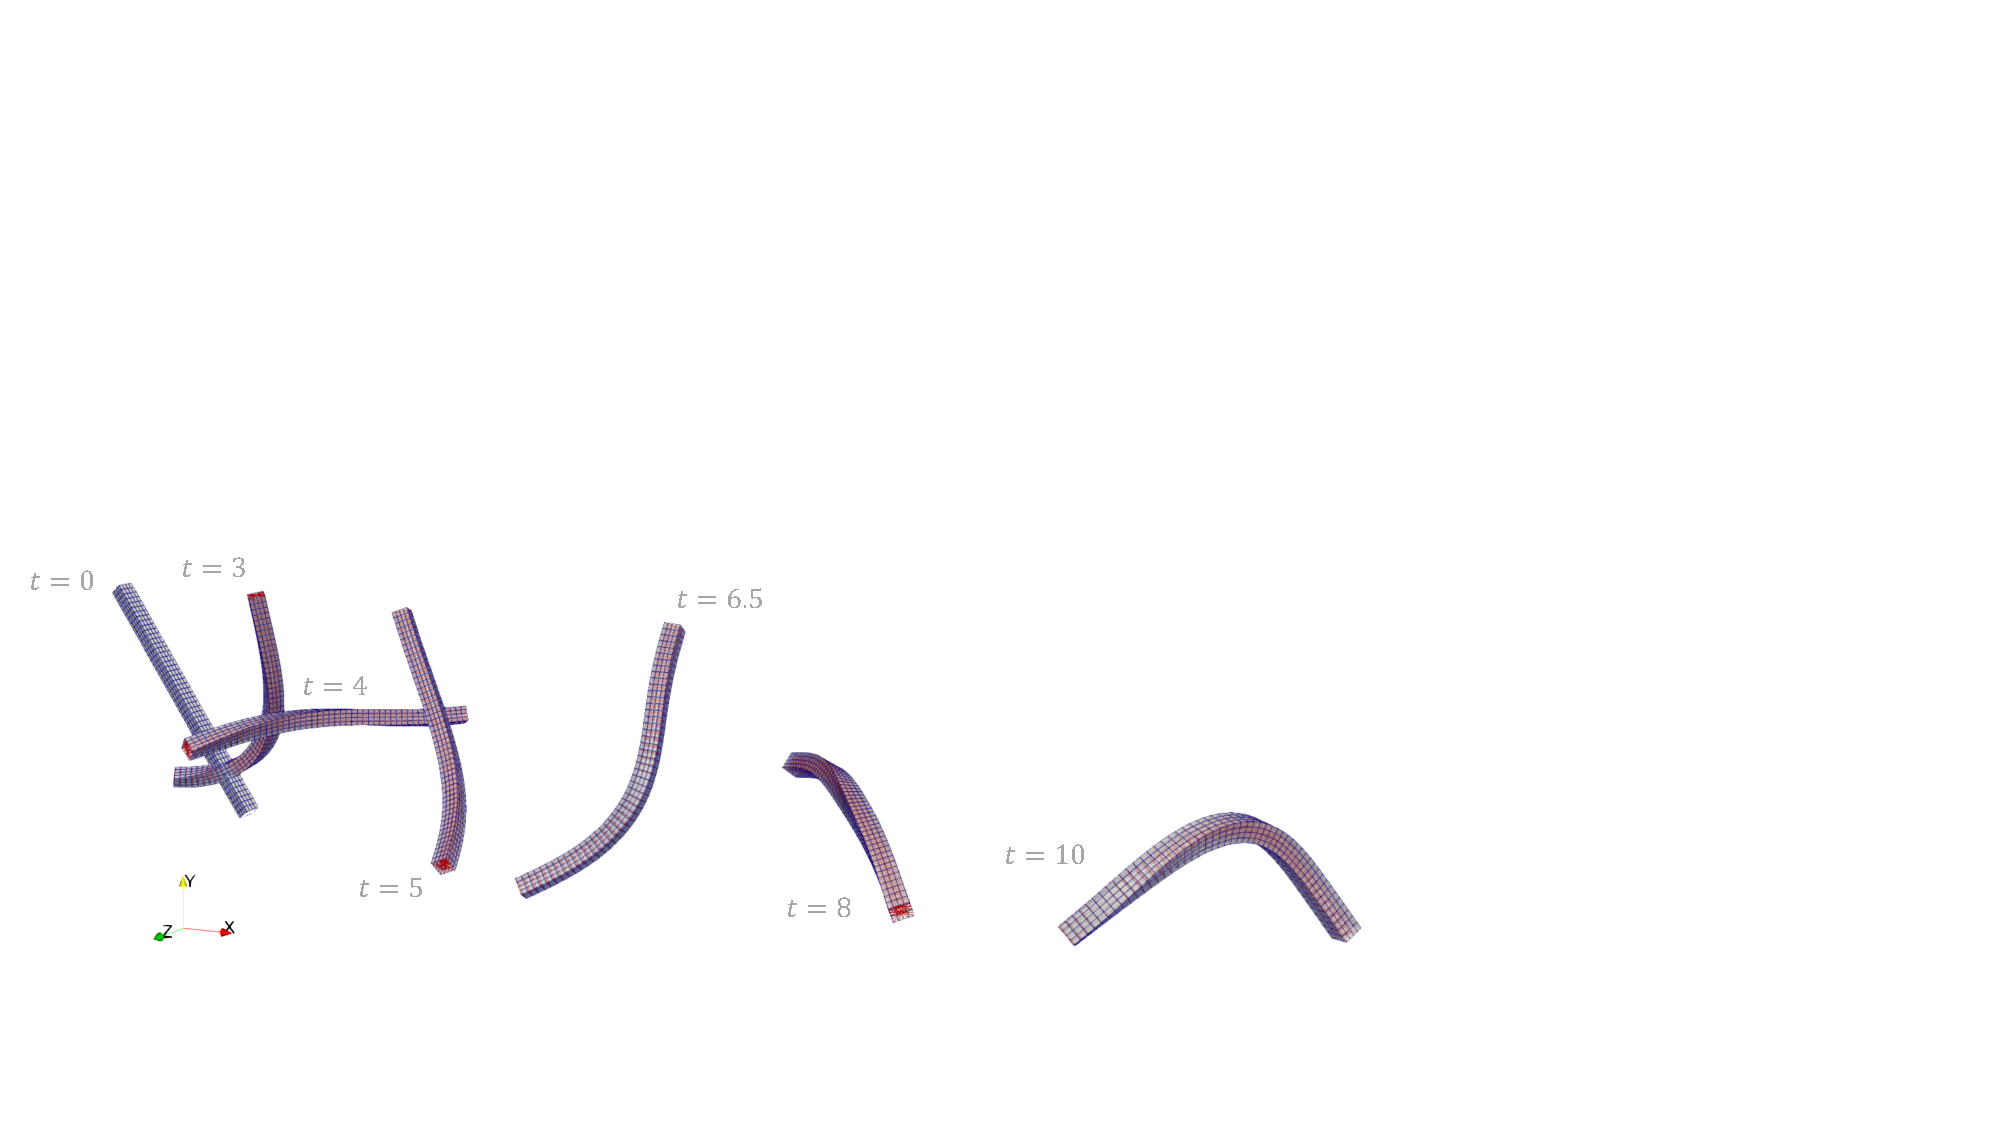
\includegraphics[width=1.\textwidth]{figs_ext/FFB_3D3.pdf}
\caption{\label{fig:org6578e1b}Free-flying structure in the 3D plane}
\end{figure}


Because the applied load is a dead force we can track the position of the center-of-gravity (CG) analytically as a verification exercise. Furthermore, the highly nonlinear nature of this problem makes it a good example to showcase the strength of accelerators for large problems and to gain insights as to when it might be better to deploy the codes in standard CPUs instead. Therefore we perform a sweep with the number of modes kept in the solution from 50 to 300, which determines the size of the system to be solved. The full modal basis is employed at 300 modes and due to the nonlinear cubic term this entails operations of the order of \(O(10^7)\) at every time step of the solution, making it a good case for accelerators. The increase in the number of modes also restricts the incremental time step used in the explicit solver to preserve stability. Table \ref{tab:org4cbfac3} shows both computational time and CG error for the planar case in two scenarios: linking  the integration time-step to the largest eigenvalue \(\lambda\) in the solution \(dt=\lambda^{-0.5}\); and fixing it to \(dt=10^{-3}\).
The error metric is defined as the L-2 norm divided by the time steps.
Computations have been carried out in AMD EPYC 7742 CPU processors and Nvidia GPU RTX 6000 at the Imperial College cluster.

\begin{table}[htbp]
\caption{\label{tab:org4cbfac3}FFB computational times in seconds and CG error}
\centering
\begin{tabular}{rllll}
Nmodes & CPU (time/err) & GPU (time/err) & CPU (time/err) & GPU (time/err)\\[0pt]
\hline
50 & 7/1.3e-1 & 9.9/1.3e-1 & 42/2.1e-2 & 58/2.1e-2\\[0pt]
100 & 9.3/5.7e-2 & 10.4/5.7e-2 & 184/1.2e-2 & 65/1.2e-2\\[0pt]
150 & 34/2.2e-2 & 14/2.2e-2 & 287/5.6e-3 & 67/5.6e-3\\[0pt]
200 & 79/2e-3 & 22/2e-3 & 421/7.2e-4 & 76/7.2e-4\\[0pt]
250 & 474/5.3e-4 & 38/5.3e-4 & 893/2.7e-4 & 94/2.7e-4\\[0pt]
300 & 1869/2.54e-5 & 111/2.54e-5 & 1869/2.54e-5 & 111/2.54e-5\\[0pt]
\hline
\end{tabular}
\end{table}

Fig. \ref{fig:org0926e7c} and \ref{fig:orgb32ed82} illustrate the times and error results in the table for the second case with fixed time step. The gain in performance from the GPU is is more impressive the larger the system to solve, and for the full modal basis the CPU takes more than 31 minutes versus the less than 2 minutes in the GPU. Computational times in the 3D problem are similar and the error on the CG position is slightly higher: for the 300 modes case, the error is \(6.9e-5\) versus the \(2.54e-5\) of the planar case.  

\url{}

\url{}

\url{}

\url{}


\subsection{XRF1}
\label{sec:org659a618}
\begin{center}
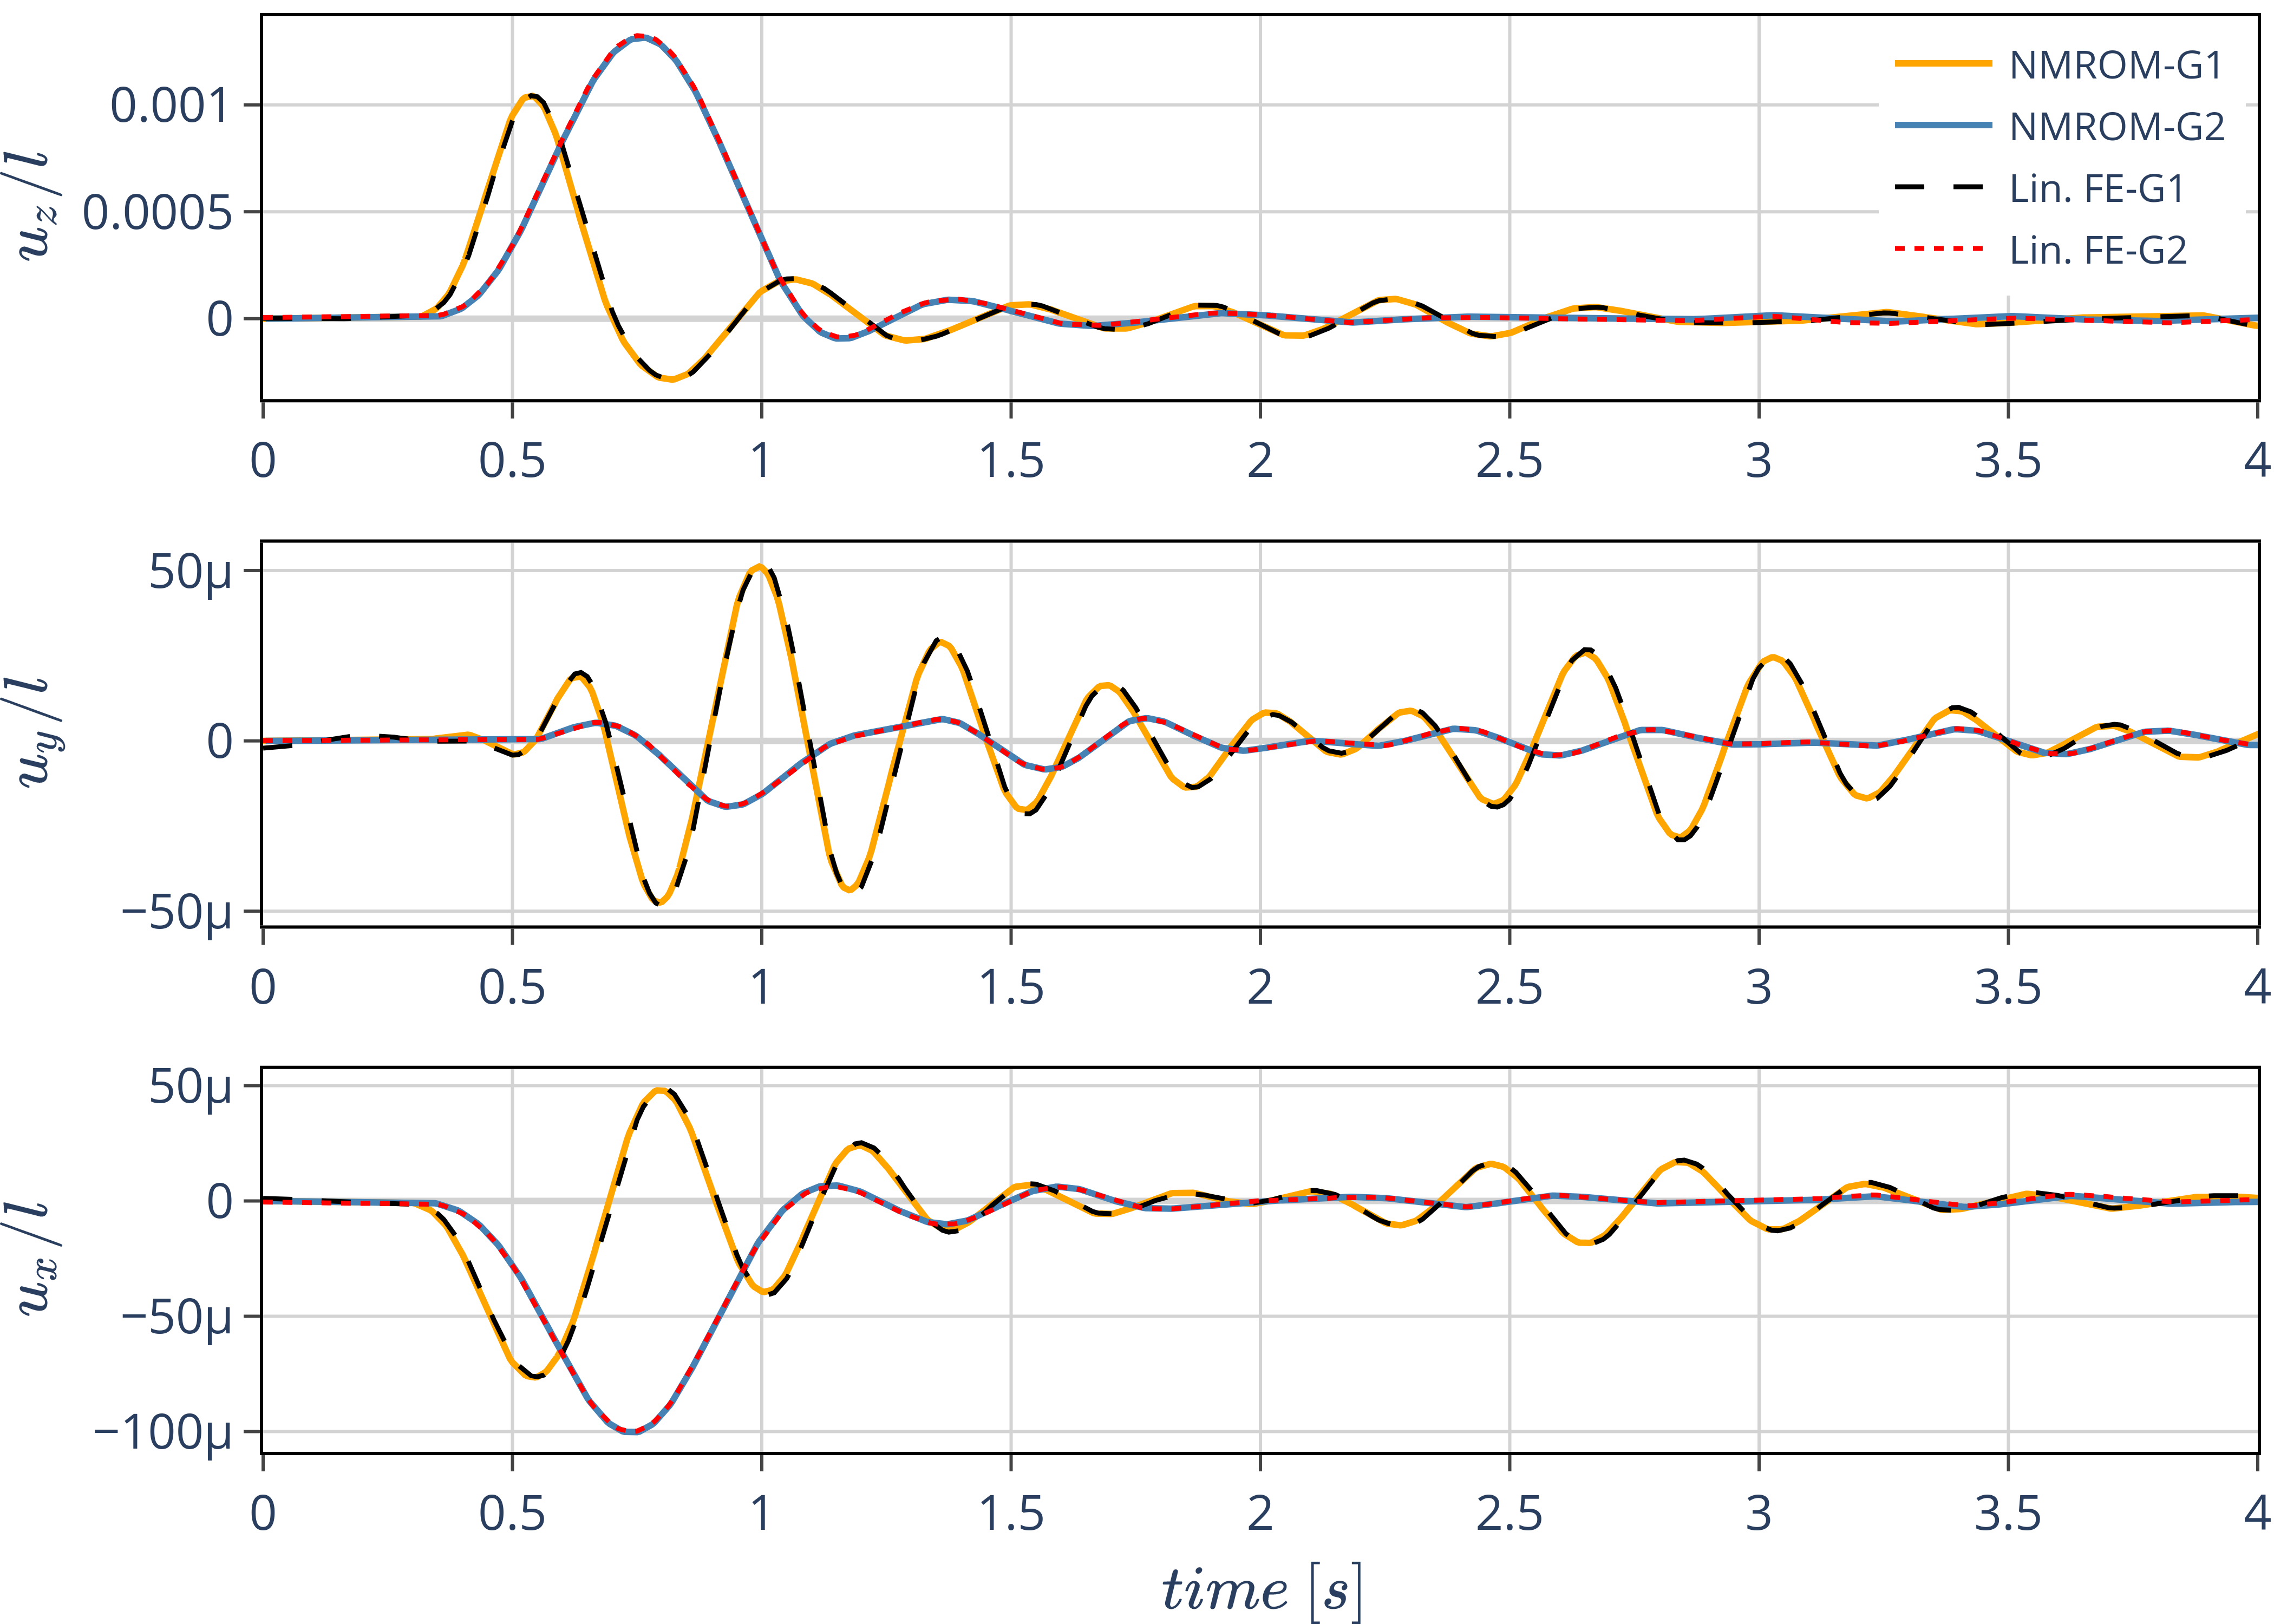
\includegraphics[width=.9\linewidth]{figs/GustXRF12.png}
\end{center}
\end{document}